\chapter{Déplacement de la voiture sur une tentacule, sans tenir compte des obstacles}
\begin{figure}[!ht]
    \centering
    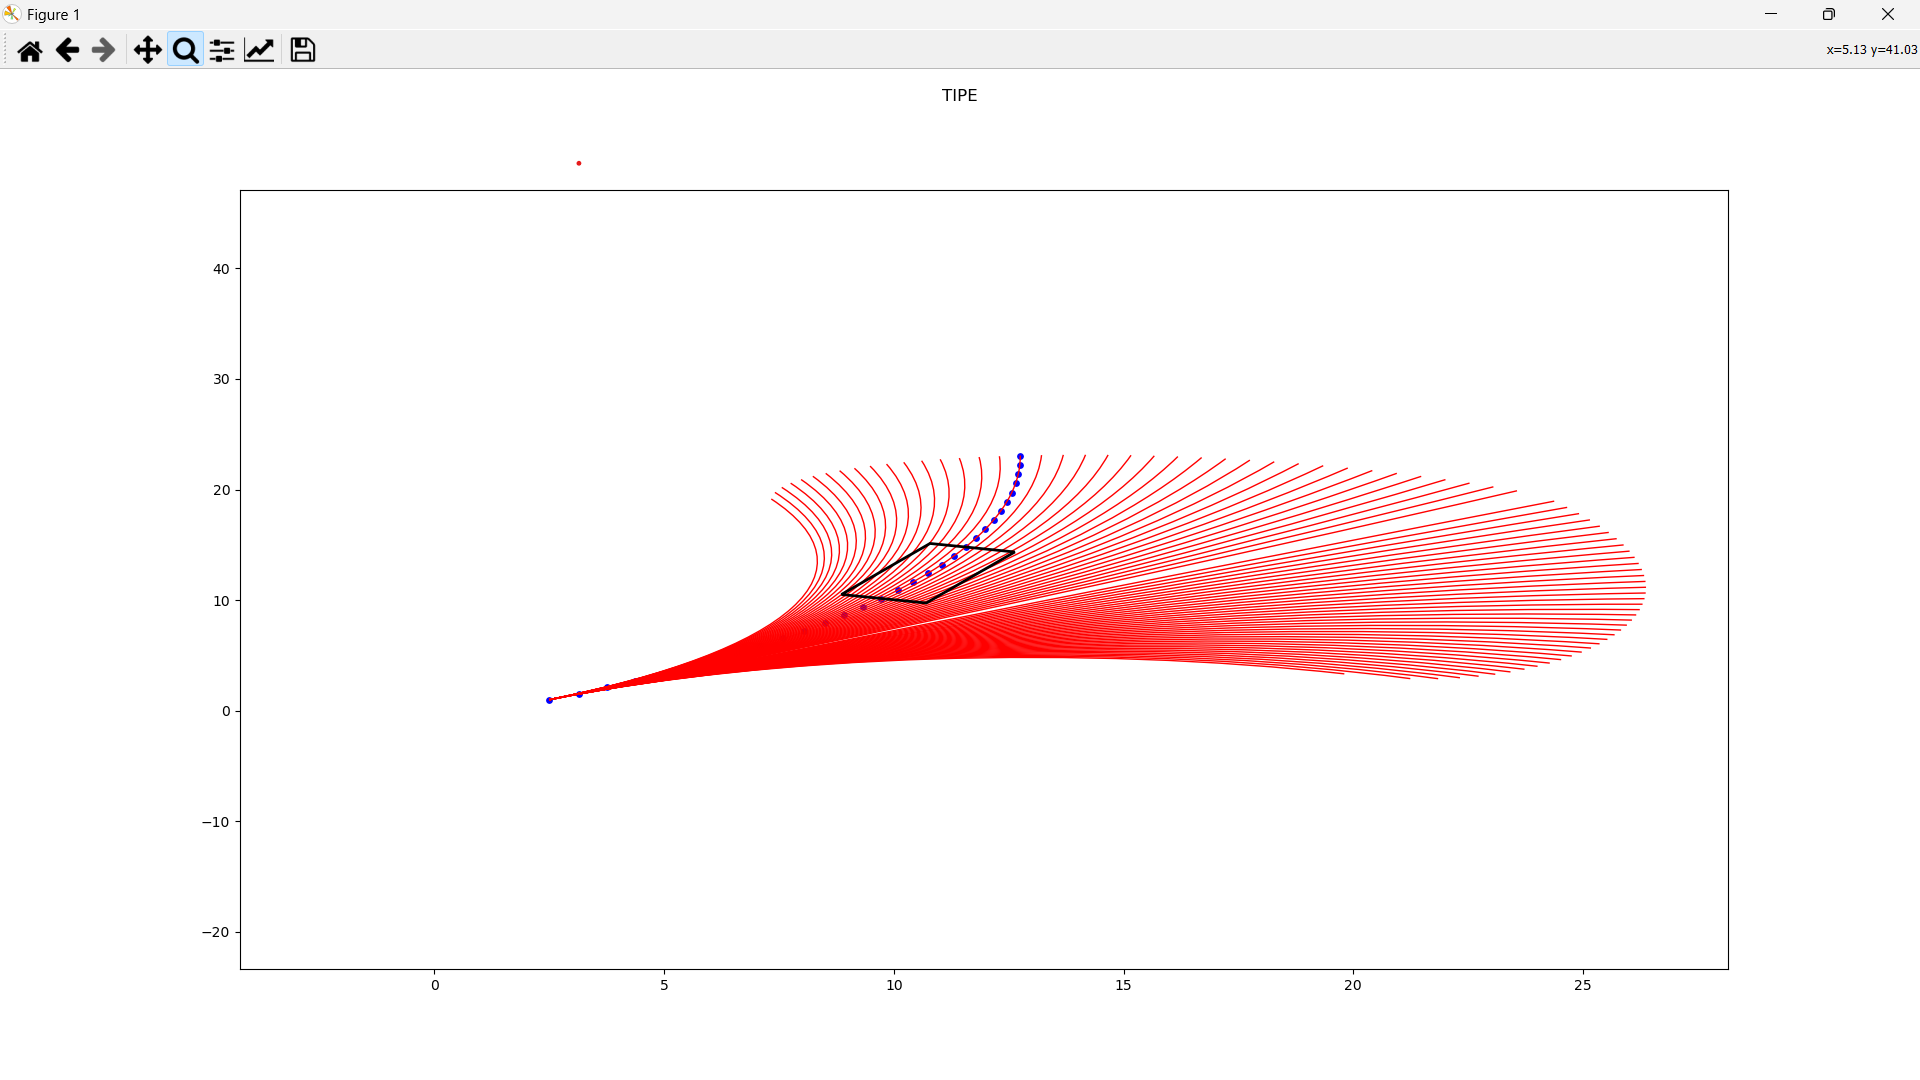
\includegraphics[scale=0.4]{deplacement successifs.png}
\end{figure}
\vspace{100pt}

\begin{mintedbox}{python}
"""
Déplace la voiture indéfiniment (selon une tentacule, puis regénération des tentacules, et suivi, et génération, etc).
"""


class Tentacule:
    """
    Objet tentacule, dépendant d'une voiture, et déterminé par son ordre et son angle de braquage.
    """
    def get_parametric(self, arc=True):
        self.precision = PRECISION
        if arc is True:
            # Définition d'un arc avec un nombre de points contrôlé
            self.patch._path = matplotlib.patches.Path.arc(self.angle_debut, self.angle_fin, self.precision)
        # Paramétrisation de la tentacule
        self.chemin = (self.patch.get_transform() - axes_ref_terre.transData).transform_path( self.patch.get_path()).cleaned().vertices[:-1][::self.signe]
        if arc is False:
            # Interpolation du chemin
            self.chemin_interpol = scipy.interpolate.interp1d(self.chemin[:, 0], self.chemin[:, 1])
            lch = len(self.chemin[:, 0])
            # Interpolation de x(t) pour faire une génération d'abscisses supplémentaires
            points = scipy.interpolate.interp1d(range(0, (lch)*self.precision, self.precision), self.chemin[:, 0])  # va jusque (lch-1)*precision inclus
            # Génération des abscisses supplémentaires avec le points(range) et des ordonnées interpolées correspondantes avec le chemin_interpol(x)
            self.chemin = np.array([[x, self.chemin_interpol(x)] for x in points(range(0, (lch-1)*self.precision, lch-1))])
        return self.chemin


class Voiture:
    """
    Objet voiture, défini par sa forme. D'autres paramètres fixes sont définis après, on pourra les mettre en paramètre plus tard si plusieurs voitures il y a.
    """
    def deplace(self):
        """
        S'il existe un chemin (suite de points), déplace la voiture suivant ce chemin.

        Raises
        ------
        erreur
            Le chemin à suivre n'est pas défini.

        Returns
        -------
        None.

        """
        try:
            new_x = self.chemin[1][0]
            new_y = self.chemin[1][1]
            vx = new_x - self.chemin[0][0]
            vy = new_y - self.chemin[0][1]
            new_angle = np.degrees(np.arctan2(vy, vx))
            self.shape_voiture.set(x=new_x - self.largeur/2, y=new_y - self.longueur/2, angle=new_angle)
            self.x, self.y, self.angle = new_x, new_y, new_angle
            self.chemin = np.delete(self.chemin, 0, 0)
        except IndexError as erreur:
            print('TENTACULE ÉPUISÉE, ON NE SAIT PLUS QUEL CHEMIN SUIVRE')
            # raise erreur

    def update_chemin(self, arc=True):
        """
        Met à jour le chemin que la voiture doit emprunter, en définissant et paramétrant la tentacule.

        Returns
        -------
        None.

        """
        self.remove_tentacules()
        self.generation_tentacules()

        ptch = self.tentacules[NUMERO_DE_LA_TENTACULE].patch  # Récupération de la forme
        self.precision = PRECISION
        if arc is True:
            # Définition d'un arc avec un nombre de points contrôlé
            ptch._path = matplotlib.patches.Path.arc(self.tentacules[NUMERO_DE_LA_TENTACULE].angle_debut, self.tentacules[NUMERO_DE_LA_TENTACULE].angle_fin, self.precision)
        # Paramétrisation de la tentacule
        self.chemin = (ptch.get_transform() - axes_ref_terre.transData).transform_path( ptch.get_path()).cleaned().vertices[:-1][: :self.tentacules[NUMERO_DE_LA_TENTACULE].signe]
        if arc is False:
            # Interpolation du chemin
            self.chemin_interpol = scipy.interpolate.interp1d(self.chemin[:, 0], self.chemin[:, 1])
            lch = len(self.chemin[:, 0])
            # Interpolation de x(t) pour faire une génération d'abscisses supplémentaires
            points = scipy.interpolate.interp1d(range(0, (lch)*self.precision, self.precision), self.chemin[:, 0])  # va jusque (lch-1)*precision inclus
            # Génération des abscisses supplémentaires avec le points(range) et des ordonnées interpolées correspondantes avec le chemin_interpol(x)
            self.chemin = np.array([[x, self.chemin_interpol(x)] for x in points(range(0, (lch-1)*self.precision, lch-1))])
        self.chemin = self.tentacules[NUMERO_DE_LA_TENTACULE].get_parametric()
        # Affichage des points que la voiture devra suivre
        plt.scatter(x=self.chemin[:, 0], y=self.chemin[:, 1], color='b', s=8)

    def generation_tentacules(self):
        """
        Génère les 80 tentacules que la voiture aura la possibilité d'emprunter.

        Returns
        -------
        None.

        """
        self.tentacules = []
        deltas = np.linspace(-self.braquage_max, self.braquage_max, 80)  # 80 est un nombre empirique de tentacules défini dans la thèse (il est bon compromis entre précision et temps de calcul)
        for k in range(1, 81):
            self.tentacules.append(Tentacule(self, k, deltas[k-1], self.axes))  # Ajout de la tentacule aux tentacules appartenant au véhicule
        for k in range(80):
            self.axes.add_patch(self.tentacules[k].patch)  # Ajout de la tentacule à la figure

    def remove_tentacules(self):
        """
        Enlève les tentacules (qui appartiennent au véhicule) de la figure.

        Returns
        -------
        None.

        """
        for tentacule in self.tentacules:
            tentacule.patch.set(visible=False)  # car si simple remove, on perd les axes de référence et c pas bon pour le blit...


class Simulation:
    """
    Classe qui gère tout l'aspect simulation : animation + gestion des objets.

    Parameters
    ----------
    voitures: list
        Liste des voitures présentes
    obstaces: list  # TODO
        liste des obstacles FIXES. Ils ne seront pas animés
    obstacles_mvt: list  # TODO
        liste des obstacles à déplacer. Fonction dévelopée plus tard
    """

    def __init__(self, voitures=[], obstacles_fixes=[], obstacles_mvt=[]):
        self.voitures = voitures
        self.obstacles_fixes = obstacles_fixes
        self.obstacles_mvt = obstacles_mvt
        self.new_tentacules = []  # liste des tentacules à afficher (blit)
        self.old_tentacules = []  # liste des tentacules qui ne sont plus d'actualité, mais qui doivent être supprimées (blit)

        for voitures in self.voitures:
            self.gestion_tentac(voiture)  # créé les tentacules de la voiture, et créé un chemin à suivre (surement inexistants jusqu'alors...)

    def animer(self, i):
        """
        Anime la figure. S'occupe de déplacer les voitures et les obstacles.
        Note : fait appel au "task-manager des tentacules" pour savoir quoi actualiser dans la figure (blit)

        Parameters
        ----------
        i : int
            Numéro d'appel de la fonction (elle est censée être appelée itérativement par une matplotlib.animation.

        Returns
        -------
        list of artists
            Liste des dessins à actualiser (blit).

        """
        # Déplace les voitures
        for voiture in self.voitures:
            voiture.deplace()
        # Déplace les obstacles
        for obstacle in self.obstacles_mvt:
            obstacle.deplace()
        try:
            # Retourne la liste des dessins à actualiser dans la figure
            # TODO : ajouter les obstacles lors de l'import de la fonctionnalité
            return [voiture.shape_voiture for voiture in self.voitures] + [tentacule.patch for tentacule in self.new_tentacules] + [tentacule.patch for tentacule in self.old_tentacules]
        finally:
            # Met juste après les valeurs adéquates à jour pour ne plus avoir à redessiner des dessins fixes (blit)
            self.old_tentacules = []  # Suppression des tentacules obsoletes, qu'on a bien effacé avec le return
            for tentac in self.new_tentacules:
                tentac.patch.set_animated(False)  # Dés-anime les nouvelles tentacules (affichées avec le return) : elles ne doivent plus bouger jusqu'à une redfinition de celles-ci
            # PROBLÈME AU NIVEAU DU BLIT : IL SEMBLERAIT QU'ON SOIT OBLIGÉ DE RETOURNER TOUTES LES TENTACULES À AFFICHER, PLUTÔT QU'UNIQUEMENT CELLES À UPDATE...
            # TODO moins urgent : résoudre ce petit problème de blit si on veut gagner un peu de temps (trace inutilement 80 tentacules...)
            # Suppression des nouvelles tentacules de la liste des dessins à actualiser
            # self.new_tentacules = []

    def gestion_tentac(self, voiture):
        """
        "Task-manager des tentacules"... Gère l'ajout et la suppression des tentacules (appartenant à la voiture *voiture*) de la figure.

        Parameters
        ----------
        voiture : Voiture
            objet voiture.

        Returns
        -------
        None.

        """
        for tentac in voiture.tentacules:  # pour mettre à jour et enlever les tentacules qui vont être supprimées
            tentac.patch.set_animated(True)  # Anime les tentacules à supprimer (elles étaient dés-animées) (blit)
            self.old_tentacules.append(tentac)  # ajout à la liste des dessins à actualiser (blit)

        voiture.update_chemin()  # suppression du système actuel de tentacules pour la voiture, puis génération de nouvelles tentacules pour la voiture

        for tentac in voiture.tentacules:  # pour mettre à jour et ajouter les tentacules qui vont être ajoutées
            tentac.patch.set_animated(True)  # anime les tentacules à ajouter (blit)
            self.new_tentacules.append(tentac)  # ajout à la liste des dessins à actualiser (blit)

\end{mintedbox}
